\section{Parsing}
\label{sec:parsing}


Il formato DXF organizza il disegno in primitive geometriche: LINE, POLYLINE, ARC, CIRCLE ecc. Queste entità sono raggruppate in layer che consentono di separare logicamente i diversi elementi del disegno (ad esempio muri, porte, finestre, arredi, testo). Oltre ai layer, il formato DXF supporta i blocchi (BLOCK), che non sono altro che componenti riutilizzabili. Sono comunemente utilizzati per rappresentare porte e finestre. Un blocco viene definito una volta all'interno del file e può essere istanziato più volte tramite entità INSERT, ciascuna con una propria posizione, scala e rotazione. Questa funzionalità è particolarmente utile per rappresentare elementi ripetuti, come porte, finestre o arredi, che compaiono più volte nella stessa planimetria.

L'obiettivo della fase di parsing è estrarre da queste primitive le informazioni geometriche necessarie alla costruzione della mesh, e collassare tutte le primitive sotto forma di segmenti per avere una rappresentazione uniforme.

Si consideri il modello CAD corretto durante il preprocessing, che presenta layer standardizzati (\texttt{A-WALL}, \texttt{A-DOOR}, \texttt{A-WINDOW}) e blocchi rinominati (\texttt{BLOCK-DOOR-1}, \texttt{BLOCK-WINDOW-1}, \ldots, \texttt{BLOCK-WINDOW-4}).

Il parsing viene realizzato in C++ mediante la libreria open source \href{https://github.com/Codelibs/libdxfrw}{libdxfrw}, che fornisce un'interfaccia per la lettura dei file DXF. La classe del parser implementa le callback necessarie per gestire i diversi tipi di entità:
\begin{minted}[frame=single]{cpp}
enum class SegmentLayer : i32 { None=0, Wall, Window, Door };
struct Segment{ glm::dvec2 start, end; SegmentLayer layer; };
	
class DRWParser : public DRW_Interface
{
public:
  virtual void addLine(const DRW_Line& data) override;
  virtual void addLWPolyline(const DRW_LWPolyline& data) override;
  virtual void addArc(const DRW_Arc& data) override;
  virtual void addInsert(const DRW_Insert& data) override;
  virtual void addBlock(const DRW_Block& data) override;
  virtual void endBlock() override;
	
  virtual void addHatch([[maybe_unused]]const DRW_Hatch* data) override {}
  virtual void addCircle([[maybe_unused]]const DRW_Circle& data) override {}
  ...
  SegmentLayer classify_layer(std::string_view name);	
  std::vector<Segment> walls, doors, windows;
};
\end{minted}

Tra le callback messe a disposizione, quelle che ci interessano maggiormente sono:
\begin{itemize}
	\item \texttt{addLine()}: viene invocata per ogni segmento (\texttt{LINE}) presente nel disegno. I due punti estremi vengono memorizzati direttamente come segmento;
		
	\item \texttt{addLWPolyline()}: per le polilinee (\texttt{LWPolyline}), si iterano i vertici della polilinea per generare una sequenza di segmenti consecutivi;
	
	\item \texttt{addArc()}: per gli archi (\texttt{ARC}), si estraggono il raggio, il punto base, l'angolo iniziale e l'angolo finale. A partire da questi dati, si calcolano i due punti estremi dell'arco, che corrispondono agli spigoli delle pareti; il segmento che li collega costituisce la rappresentazione della porta;
	
	\item \texttt{addInsert()}, \texttt{addBlock()}: questi metodi gestiscono le istanze dei blocchi. Le primitive all'interno di un blocco sono definite in coordinate locali; è necessario applicare una trasformazione per rappresentarli in world space.
	
\end{itemize}

Per distinguere i segmenti in base alla loro semantica, si utilizza il nome del layer:

\begin{minted}[frame=single]{cpp}
SegmentLayer classify_layer(std::string_view name)
{
  if (name.compare("A-DOOR") == 0)    return SegmentLayer::Door;
  if (name.compare("A-WALL") == 0)    return SegmentLayer::Wall;
  if (name.compare("A-WINDOW") == 0)  return SegmentLayer::Window;
  return SegmentLayer::None;
}
\end{minted}

Analogamente anche per i blocchi:
\begin{minted}[frame=single]{cpp}
void DRWParser::addBlock(const DRW_Block& data)
{
  if(data.name.contains("BLOCK-DOOR") || 
     data.name.contains("BLOCK-WINDOW"))
  {}
}
\end{minted}

Per questo motivo rinominare correttamente layer e blocchi è fondamentale.

Questa classificazione per layer e per blocco è fondamentale perché, come si vedrà successivamente, consente di trattare in modo differenziato pareti, porte e finestre durante la fase di estrusione.

Per verificare la correttezza del parsing, utilizziamo uno script Python per fare il plot del grafico:
\begin{figure}[htbp]
	\centering
	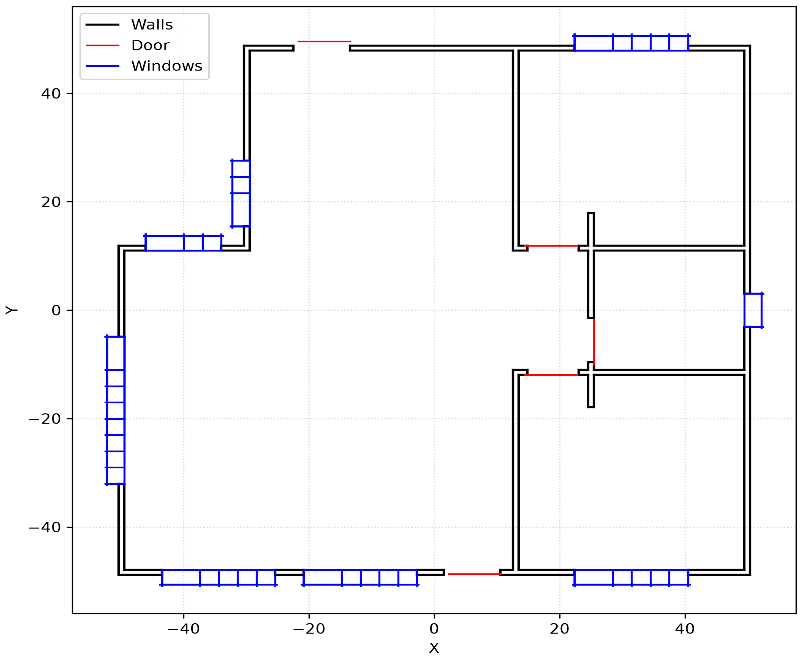
\includegraphics[width=0.7\textwidth]{images/02_geometry_processing/parsing.png}
	\caption{Plot dei segmenti}
	\label{fig:parsing}
\end{figure}